\section{Theoretical Background}
Establishing a foundational understanding of the underlying technologies and review the current state of the art in digital investigations is crucial to be able to develop a methodology for IoT behavioural reconstruction. This section provides the theoretical framework necessary to contextualize the proposed research, mapping the technical landscape of connected devices and identifying the existing gaps in current forensic methodologies.

\subsection{IoT Architectures}
To successfully analyse the network behaviour of an IoT device, it is first necessary to understand the structural paradigm in which it operates. Contrary to the traditional network based on standard endpoints (desktop computers and servers), the IoT ecosystem is highly distributed and heterogeneous. Academic consensus generally model the IoT architecture across three primary tiers: the Edge (or Perception) Layer, the Fog (or Network/Gateway) Layer, and the Cloud (or Application) Layer \cite{WinSystems2020}. To address increasing complexity, standard bodies such as the International Telecommunication Union (ITU-T) have formalized a four-layer model (Device, Network, Service Support and Application layers). \cite{ITUTY2060}.

Understanding this layered architecture is critical for digital forensics as it defines where data is generated, how it is encapsulated in transit and where investigators can feasibly deploy network capture tools.

\subsubsection{Edge, Fog, Cloud}

This hierarchical structure addresses the challenges of IoT by distributing processing and storage responsibilities across these layers. This allows the IoT system to provide locally real-time responsiveness while leveraging the vast analytical power of the cloud. 

\begin{itemize}
	
	\item \textbf{Edge Layer:} Lowest tier of the architecture, consisting only of hardware deployed in the environment. Includes elements such as sensors, which gather data, and actuators, which perform physical actions. This type of devices have minimal processing power as well as a highly volatile memory. Their objective is to interact with the physical world but rely on upper layers for complex processing and long-term storage. 
	
	\item \textbf{Fog:} Acts as the bridge between both layers, the local smart environment and the wider internet. Consists of network gateways, local routers and edge computing nodes \cite{Bonomi2012}. Since Edge devices use low-power, non-IP communication protocols, the gateway has  responsibility of translating these signals into standard IP traffic for internet transit. Furthermore, it often performs data normalization, ensuring that sensor formats are unified before transmission. This point is vital for digital forensics since it offers visibility of all localized device behaviours and its outbound communications before they are integrated to the cloud. 
	
	\item \textbf{Cloud:} Most widely adopted architecture across industries. A cloud platform consists of distributed servers and storage resources accessible over the internet. These systems provide virtually unlimited computing and storage, elastic scalability, centralized data aggregation and high data analytics capabilities. 
\end{itemize}

The most important element for digital forensics in this architecture is the Fog layer since it is the translator and the routing point for the smart environment with the cloud. 

\begin{figure}[H]
	\centering
	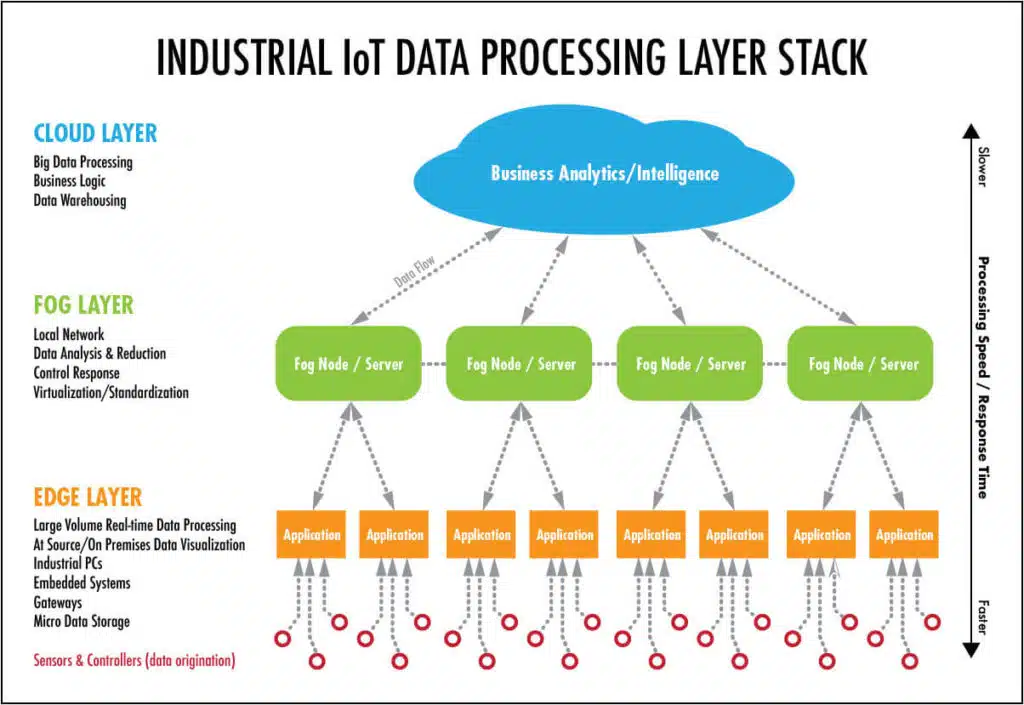
\includegraphics[width=0.7\linewidth]{Images/theory/iot_fog_edge}
	\caption{Edge, Fog, Cloud Layers architecture \cite{WinSystems2020}}
	\label{fig:iotfogedge}
\end{figure}

\subsubsection{ITU-T Y.2060}
ITU framework focused on a four vertical stack supported by two horizontal management and security capabilities that span accross all layers.

\textbf{The Four-Layer Architecture} \newline

\begin{enumerate}
	\item \textbf{Application Layer:} The top tier where specific IoT applications reside. It interacts with the lower layers to consume processed data and provide services to the end-user.
	
	\item \textbf{Service Support and Application Support Layer:} Acts as a middleware. It provides common capabilities used by many applications (Service Support),and capabilities tailored to a particular industry or application type (Specific Support).
	
	\item \textbf{Network Layer:} Responsible for communication and connectivity. It handles the Networking Capabilities (routing and transport) and Access Capabilities (connecting devices to the core network).
	
	\item \textbf{Device Layer:} The physical foundation. It includes the "Things" (sensors and actuators). Devices can interact with the network directly or through a \textbf{Gateway} if they use low-power, non-IP protocols.
\end{enumerate}

\textbf{Cross-Layer Capabilities} \newline

A key feature of the ITU architecture is that it identifies two functions that must exist at every single level of the stack:

\begin{itemize}
	\item \textbf{Management Capabilities:}  Covers fault management, configuration, accounting, performance, and security management (FCAPS) across the entire system.
	
	\item \textbf{Security Capabilities:} Ensures data privacy, device authentication, and communication integrity at every point where data is handled or moved.
\end{itemize}

\begin{figure}[H]
	\centering
	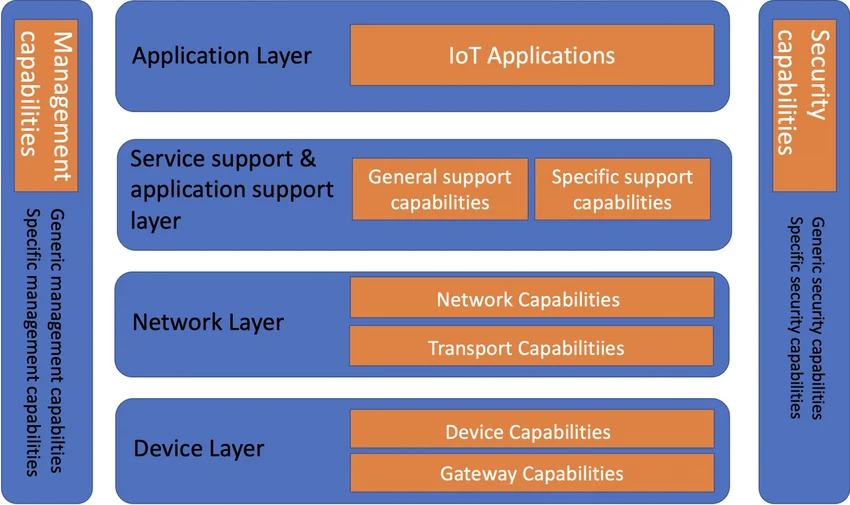
\includegraphics[width=0.7\linewidth]{Images/theory/iot_itut2060}
	\caption{ITU-T Y.2060 Layered Architecture \cite{Albreem2022}}
	\label{fig:iotitut2060}
\end{figure}


The ITU model also formalizes the Gateway as a specific functional entity within the Device Layer. This confirms the claim that the Fog/Gateway layer is the most important point for digital forensics, as it is the first point where device specific data is aggregated and managed. 

\subsection{Network Protocols}

\subsubsection{Message Queuing Telemetry Transport}
 
 Message Queuing Telemetry Transport (MQTT) was originally developed by IBM in 1999 and it is currently maintained as an OASIS standard. It is one of the most widely adopted messaging protocols in the IoT ecosystem \cite{RFC9431}. It is specifically designed for constrained devices operating on low-bandwidth, high-latency or unreliable networks. It is the standard for smart home sensor communication. 

Contrary to web protocols such as HTTP, MQTT operates on a \textbf{Publish/Subscribe} architectural model. IoT devices do not communicate directly with one another, all communications are routed through a central server known as \textbf{MQTT Broker}, which typically resides at the Fog layer or in the Cloud. Devices publish messages called topics and the rest of devices can subscribe to these topics to receive updates. 

The protocol runs over the TCP/IP stack and exhibits highly specific identifiable network footprints:

\begin{itemize}
	\item \textbf{Standardized Ports:} By default, unencrypted traffic operate over TCP port 1883. While encrypted (MQTT over TLS/SSL) uses port 8883. Identifying persistent TCP streams on these ports is the primary method for isolating MQTT traffic from background network noise.
	
	\item \textbf{Keep-Alive Mechanisms:} To maintain the persistent TCP connection without constantly sending data, MQTT clients periodically transmit \texttt{PINGREQ} (Ping Request) packets to the broker, which responds with a \texttt{PINGRESP} (Ping Response). These periodic and uniformly sized packets establish a critical baseline of "normal" device behavior. An interruption in this keep-alive rhythm often indicates device failure, a reboot, or a targeted denial-of-service attack.
	
	\item \textbf{Quality of Service (QoS) Flows:} MQTT defines three QoS levels (0: At most once, 1: At least once, 2: Exactly once) that dictate the reliability of message delivery. Higher QoS levels require a multi-step acknowledgment handshake (e.g., \texttt{PUBACK}, \texttt{PUBREC}, \texttt{PUBREL}). For an investigator, observing these acknowledgment sequences in the traffic flow provides insight into the importance and type of data being transmitted, even if the payload is encrypted \cite{Hassan2021}.
\end{itemize}

\begin{figure}[H]
	\centering
	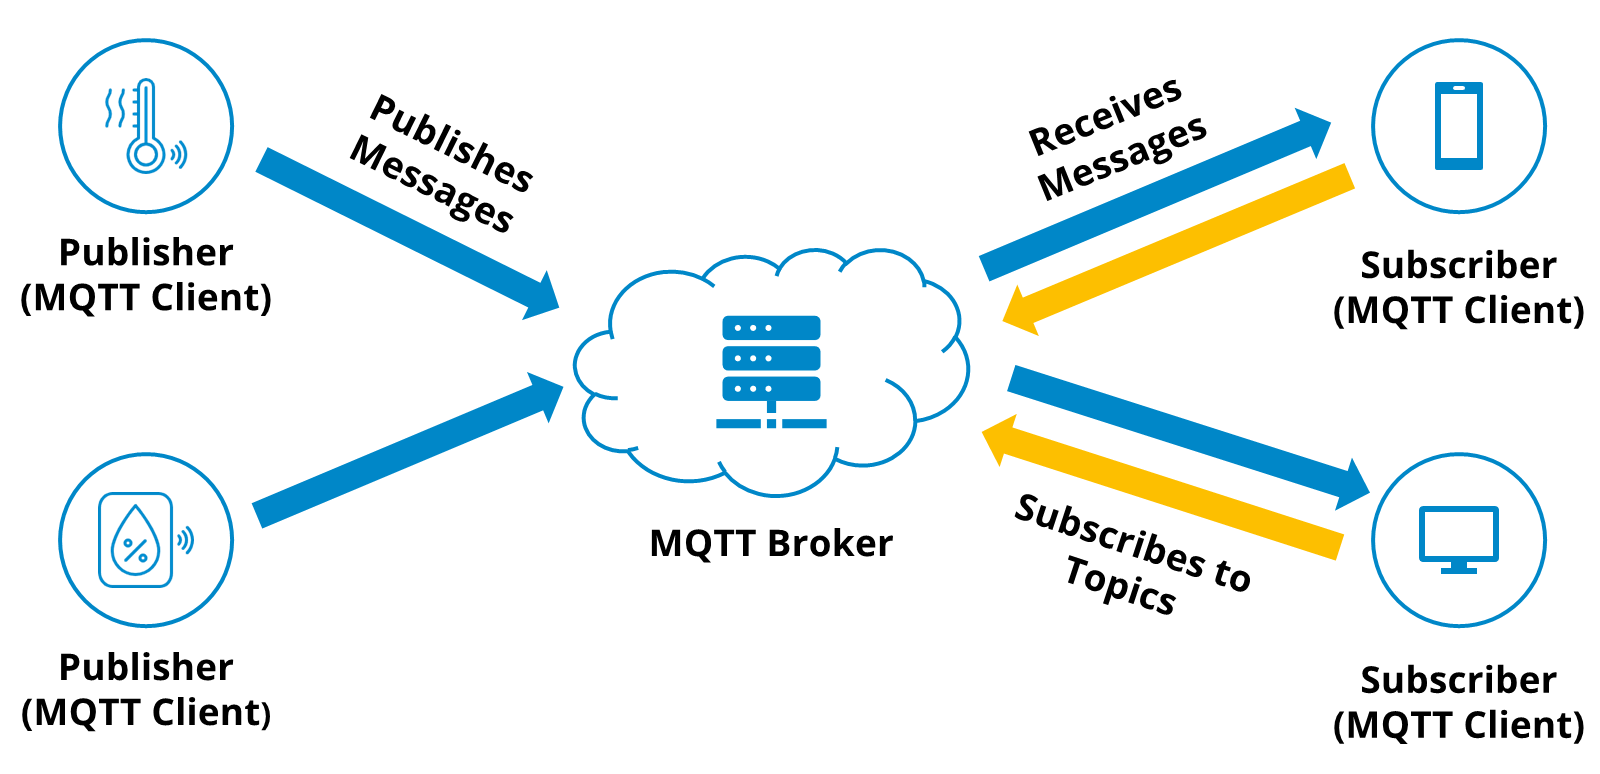
\includegraphics[width=0.7\linewidth]{Images/theory/mqtt}
	\caption{MQTT work schema \cite{Manubes2023}}
	\label{fig:mqtt}
\end{figure}

Modern security practices strongly mandate the use of MQTT over TLS (port 8883). Consequently, modern IoT forensic methodologies cannot rely on reading the payload. Investigators should use metadata such as frequency of publish packets, the size of the encrypted payloads and the keep-alive intervals to infer the device's physical state. 

\subsubsection{Constrained Application Protocol}
The Constrained Application Protocol (CoAP) was developed by the Internet Engineering Task Force (IETF) to serve as a lightweight, specialized alternative to HTTP for constrained devices \cite{RFC7252}. Operating on a traditional client-server RESTful architecture, CoAP allows IoT devices to utilize familiar web methods (GET, POST, PUT, DELETE) while maintaining an extremely low overhead suitable for low-power microcontrollers.

The most significant distinction between CoAP and MQTT is the transport layer. While traditional HTTP and MQTT rely on the connection-oriented Transmission Control Protocol (TCP), CoAP is designed to operate primarily over the connectionless User Datagram Protocol (UDP). This architectural choice drastically alters the network artifacts available for behavioral reconstruction:

\begin{itemize}
	\item \textbf{Connectionless Traffic Analysis:} By default, CoAP operates over UDP port 5683, while encrypted CoAP traffic utilizes UDP port 5684. Because UDP lacks the traditional three-way handshake (SYN, SYN-ACK, ACK) and connection teardown (FIN) of TCP, investigators cannot rely on standard network flow boundaries to determine when a device session begins or ends. Instead, forensic analysts must look for specific temporal clusters of UDP packets to infer interaction.
	
	\item \textbf{Application-Layer Reliability Mechanisms:} To compensate for the unreliability of UDP, CoAP implements its own lightweight reliability mechanisms directly within the message header. CoAP frames are categorized into four distinct types: Confirmable (CON), Non-confirmable (NON), Acknowledgement (ACK), and Reset (RST). From a network analysis perspective, observing the ratio and timing of CON to ACK packets provides excellent behavioral indicators. For example, a sudden spike in unacknowledged CON messages may indicate a device experiencing a network failure, a localized jamming attack, or a disrupted cloud backend.
	
	\item \textbf{Message IDs and Tokens:} Because UDP packets can arrive out of order, CoAP utilizes Message IDs for detecting duplicates and matching ACKs and Tokens for matching asynchronous requests and responses. These identifiers act as critical metadata threads, allowing them to form together a chronological sequence of requests and responses even when the surrounding network environment is highly congested.
\end{itemize}

Modern security standards mandate that CoAP payloads should be encrypted. CoAP utilizes Datagram Transport Layer Security (DTLS) on port 5684. Once DTLS is established, the specific RESTful commands are obscured. Consequently, the forensic methodology must pivot entirely to metadata analysis as with MQTT. Some examples of techniques are correlating the size of the DTLS payload, the direction of the traffic, and the frequency of the UDP datagrams to classify the physical action the device is executing.

\subsubsection{HTTP/HTTPS \& TLS/SSL}

The traditional Hypertext Transfer Protocol (HTTP) and its secure counterpart (HTTPS) remain fundamental to the broader IoT ecosystem. HTTP relies on a client-server RESTful architecture operating over the Transmission Control Protocol (TCP). In IoT environments, HTTP is normally used by high-bandwidth devices, administrative web interfaces and the critical Fog layer gateways and Cloud layer vendor backends. 

As the rest of protocols, HTTPS is mainly used for security concerns. This protocol version obscures he payload and the specific URL paths accessed by the device. To reconstruct device behaviour network forensic methodologies must pivot to analysing the cryptographic handshakes and contextual flow metadata: 

\begin{itemize}
	\item \textbf{Server Name Indication (SNI):} During the initial TLS handshake, before the encrypted tunnel is fully established, the client typically transmits a \texttt{ClientHello} message in cleartext. This message frequently contains the Server Name Indication (SNI) extension, which reveals the plaintext domain name the device is attempting to contact. The SNI is arguably the most valuable artifact in encrypted traffic, as it immediately identifies the device's manufacturer, its intended cloud backend, and often its specific function.
	\item \textbf{Flow Duration and Throughput Profiling:} Because the RESTful commands are encrypted, investigators must infer the device's action by analyzing the shape of the TCP flow. A short, low-byte TCP flow likely represents a routine heartbeat or authentication check with the cloud. Conversely, a prolonged TCP session with massive upstream byte transfer strongly indicates active video streaming or data exfiltration.
	\item \textbf{TLS Fingerprinting:} Because IoT devices utilize highly specific, embedded operating systems and libraries (such as OpenSSL or mbedTLS), they negotiate TLS connections in highly predictable ways. By analyzing the specific combination of cipher suites, supported elliptic curves, and TLS extensions offered during the \texttt{ClientHello}, investigators can create a cryptographic fingerprint of the device. This allows analysts to definitively identify the type of IoT device generating the traffic, even when the traffic is fully encrypted and background noise is high.
\end{itemize}


\subsection{Challenges in IoT Forensics}
As previously introduced in the previous section, conducting digital forensics within the IoT ecosystem presents a unique set of obstacles that make classical device based methodologies ineffective. To successfully investigate these environments, analysts must thoroughly understand these limitations and apply workarounds mainly based on network forensics. The primary identified challanges are listed below:

\begin{itemize}
	\item \textbf{Ephemeral Data and Constrained Storage:} The majority of operational data and cryptographic keys are held in volatile memory (RAM) and are permanently lost upon a device reboot. Furthermore, due to constrained storage capacities, any existing flash memory logs are rapidly overwritten in a continuous loop. 

	\item \textbf{Proprietary Hardware and Interfaces:} Devices rely on closed-source custom firmware and lack standardized physical data extraction interfaces (such as SATA or USB ports), acting as inaccessible "black boxes".
	
	\item \textbf{The Encrypted Payload Barrier:} To protect user privacy, modern IoT protocols implement encryption methods. This results in Deep Packet Inspection (DPI) being obsolete, as investigators cannot read the payload contents.
	
	\item \textbf{Semantic Gap in Behavioral Translation:} There is a fundamental disconnect between raw, encrypted network data and physical device actions, making it difficult to map a TCP flow to a real-world event (e.g., a smart lock opening). 
	
	\item \textbf{Volume and Background Noise:} IoT devices are highly chatty, constantly generating benign ambient noise such as keep-alive messages, NTP synchronizations, and heartbeat signals to cloud servers. 
	
	\item \textbf{Time Synchronization and Blurry Boundaries:} The existence of multiple data sources with varying time zones, clock drifts, and blurry network perimeters complicates the generation of a unified chronological timeline. 
	
	\item \textbf{Protocol Heterogeneity and Network Fragmentation:} Unlike traditional IT networks that primarily rely on standard TCP/IP over Ethernet or Wi-Fi, the IoT ecosystem is highly fragmented. A single smart home may simultaneously utilize different protocols to implement their services. This requires investigators to deploy multiple specialized sniffing tools and gateways to capture the full spectrum of device communications, complicating the unified capture process.
	
	\item \textbf{Cloud Dependency and Data Fragmentation:} Many IoT architectures rely heavily on cloud processing. Consequently, local device-to-device interactions are frequently routed out to vendor-controlled external servers before executing a local action. Local network captures rely on analyzing encrypted outbound streams rather than direct, localized command-and-control traffic.
\end{itemize}

These constraints demonstrate that traditional forensics techniques and procedures are incompatible with the IoT ecosystem. Because investigators cannot reliably extract persistent data from physical edge devices, nor easily decrypt in transit communications, the network gateway emerges as the most critical vantage point for evidence acquisition. 

However, the presence of an encrypted payload leads on an insufficient capturing of network traffic. To successfully reconstruct a chronological timeline of events, investigators must pivot from content-based analysis to context-based analysis. This requires the development and application of advanced methodologies capable of identifying specific devices which objective is to guess the state of the device based on the encrypted network flow and its metadata. This is known as IoT traffic fingerprinting. 


\subsection{IoT Traffic Fingerprinting}
To bridge the gap between encrypted network flows and physical device events, investigators use a methodology known as IoT traffic fingerprinting. \textbf{Fingerprinting} is the process of passively observing network traffic to extract a unique set of features or metadata (a fingerprint) that can reliably identify a specific device, its operating system, or its current physical state \cite{Miettinen2017}.

In traditional IT environments, fingerprinting often relies on deep packet inspection (DPI) or active scanning. An example of active scanning can be sending tailored ICMP or TCP SYN packets to observe the target's response. However, because IoT devices are resource-constrained and easily disrupted by active scanning, and their payloads are predominantly encrypted, modern IoT fingerprinting relies exclusively on the passive statistical analysis of traffic flows.

IoT fingerprinting can be divided into two distinct phases: Device-Level Fingerprinting and Behavioral and State Fingerprinting.

\subsubsection{Device-Level Fingerprinting}
The first objective when capturing network traffic must be to identify the devices present in the environment. Device fingerprinting relies on the highly repetitive and single-purpose nature of IoT hardware. In general, most IoT devices have different hardware components as well as forming part of different cloud architectures. For this reason, IoT network footprints are usually highly distinct \cite{Sivanathan2019}. To classify device types, investigators analyze:

\begin{itemize}
	\item \textbf{Protocol Signatures:} Identifying the specific combination of protocols used. The use of a port or another indicates which protocol is implemented by the device. 
	\item \textbf{Initialization and DNS Patterns:} When IoT devices boot or reconnect to a network, they frequently perform specific DNS queries to vendor-controlled domains for time synchronization or for cloud registration). Extracting these plaintext queries from DNS logs (typically UDP port 53) provides immediate, high-fidelity device attribution.
	\item \textbf{TLS Handshake Metadata:} If TLS is used, as discussed in Section 2.1, extracting the Server Name Indication (SNI) and mapping the supported cipher suites negotiated during the \texttt{ClientHello} phase allows investigators to uniquely identify the device's embedded operating system \cite{Miettinen2017}.
\end{itemize}

\subsubsection{Behavioral and State Fingerprinting}
Once the devices involved in the capture are identified, the focus turns to behavioral reconstruction. Behavioral fingerprinting seeks to relate variations in the network flow to specific physical actions. For example, differentiating between a camera standing by, actively recording, or being rebooted. Because the payloads are encrypted, this identification relies heavily on flow-level statistics. The most crucial characteristics utilized for behavioral fingerprinting include:

\begin{itemize}
	\item \textbf{Packet Length and Size Distribution:} Specific actions trigger specific payload sizes. For example, a smart lock communicating an "unlock" command will consistently generate a highly specific, small packet size compared to a camera streaming a variable bitrate video.
	\item \textbf{Inter-Arrival Time (IAT):} IAT measures the time elapsed between consecutive packets in a flow. IoT devices often exhibit highly periodic IATs due to automated heartbeat messages. A sudden, dense clustering of packets typically signifies a triggered physical event or an ongoing cyberattack.
	\item \textbf{Flow Volume and Duration:} Analyzing the total bytes transferred over a specific window of time helps categorize the device's current state. For example, a baaseline state may show 5 KB transferred per minute, while an active data exfiltration or firmware update event may spike to several megabytes per minute.
\end{itemize}

By establishing a baseline of these statistical features during normal operation, investigators can create and define a classification of the known states for each device. When an anomaly or malicious event occurs, the resulting traffic spike can be matched against this classification, allowing the investigator to reconstruct a timeline of the device's physical behaviour without ever decrypting the underlying data.


\subsection{NIST Guidelines}
To successfully apply the traffic fingerprinting and behavioural reconstruction methodologies previously discussed, a "ground truth" must be established. This ground truth is mostly based on reconstructing a forensic timeline, which basically relies on the ability to distinguish between normal operational traffic, user-triggered physical events, and malicious anomalies. To define these baselines, the cybersecurity sector heavily rely on the standards and publications made by important institutions. A great example to follow, are the baselines established by the National Institute of Standards and Technology (NIST).

NIST has published several highly influential frameworks that dictate how IoT devices should be designed, how they should behave on a network, and how their traffic has to be managed. For the purposes of network-based IoT forensics, NIST guidelines are particularly relevant: Foundational Device Capabilities and Network-Layer Behavioral Whitelisting.

\subsubsection{Foundational Device Capabilities (NISTIR 8259)}
The NIST Interagency Report (NISTIR) 8259 series \cite{NISTIR8259} provides guidance for manufacturers and their supporting third parties as they conceive, design, test, sell and support IoT devices across their spectrum of customers. From a forensic perspective, the most critical mandate within this framework is the IoT Device Cybersecurity Capability Core Baseline \cite{NISTIR8259A}.

\begin{figure}[H]
	\centering
	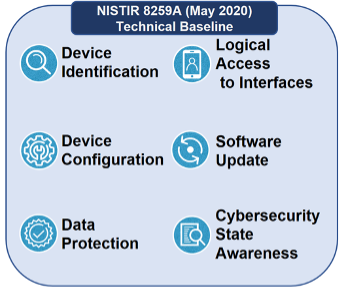
\includegraphics[width=0.45\linewidth]{Images/theory/NIST-8259-A}
	\caption{NISTIR8259A capabilities \cite{NISTIR8259A}.}
	\label{fig:nist-8259-a}
\end{figure}


NIST dictates that an IoT device should have a strictly defined, predictable set of network interactions. The document outlines the capability of IoT devices to restrict and manage local and network accesses. For example, it defines that an IoT device should only communicate with specific authorized endpoints using specific protocols. By mandating that manufacturers document these expected behaviors, NIST implicitly validates the core premise of network-based IoT forensics. This means that any deviation from this documented predictable network footprint strongly indicates a physical state change, a configuration error, or a security compromise.

Furthermore, the 8259A baseline mandates that devices must implement a \textbf{Device Identification} method such as a logical identifier like a MAC address or UUID. This is important for the forensic investigator since the identification of this unique identifier is the first step in the timeline reconstruction.

There are some other capabilities that must be defined that can be important for a forensic investigation:

\begin{itemize}
	\item \textbf{Data Protection:} NIST mandates that manufacturers must use cryptography to protect data in transit. For this reason, Deep Packet Inspection is not the solution, making feature extraction necessary.
	
	\item \textbf{Software Update:} Devices must be able to receive Over-The-Air firmware updates. This has a highly distinct network footprint since the device must perform a DNS request, followed by a massive TCP data flow. 
	
	\item \textbf{Cybersecurity State Awareness:} The device should be able to report its status and special events such as errors, crashes, unauthorized access attempts to the cloud or local admin. This means that devices will automatically generate automated network traffic when something goes wrong. The identification or monitoring of these notifications is important since a spike in State Awareness traffic can indicate the existence of an ongoing attack. 
\end{itemize}


\subsubsection{Network-Layer Monitoring and MUD (NIST SP 1800-15)}
Device logs are unreliable as previously discussed in Section 2.2. For this reason, NIST Special Publication 1800-15 \cite{NISTSP180015} defines the concept of Manufacturer Usage Description (MUD) specificagtion for IoT devices. The objective is to ensure that manufactures can indicate the network communications that a device requires to perform its intended function. When MUD is used, the network will automatically permit the IoT device to send and receive only the traffic it requires to perform as intended, and the network will prohibit all other communication with the device, increasing the device’s resilience to network-based attacks. 

This standard specifies a data model, a JSON-formatted file, to describe a set of access control entries representing allowed communications of an IoT device on the network. It also defines in-band mechanisms by which an IoT device can signal to the network supplying the MUD model that indicates what access and protection the device needs. Devices typically broadcast the URL of their MUD file in plaintext during the initial network boot sequence. The following image is an example of the MUD profile for a TP Link Camera. 


\begin{figure}[H]
	\centering
	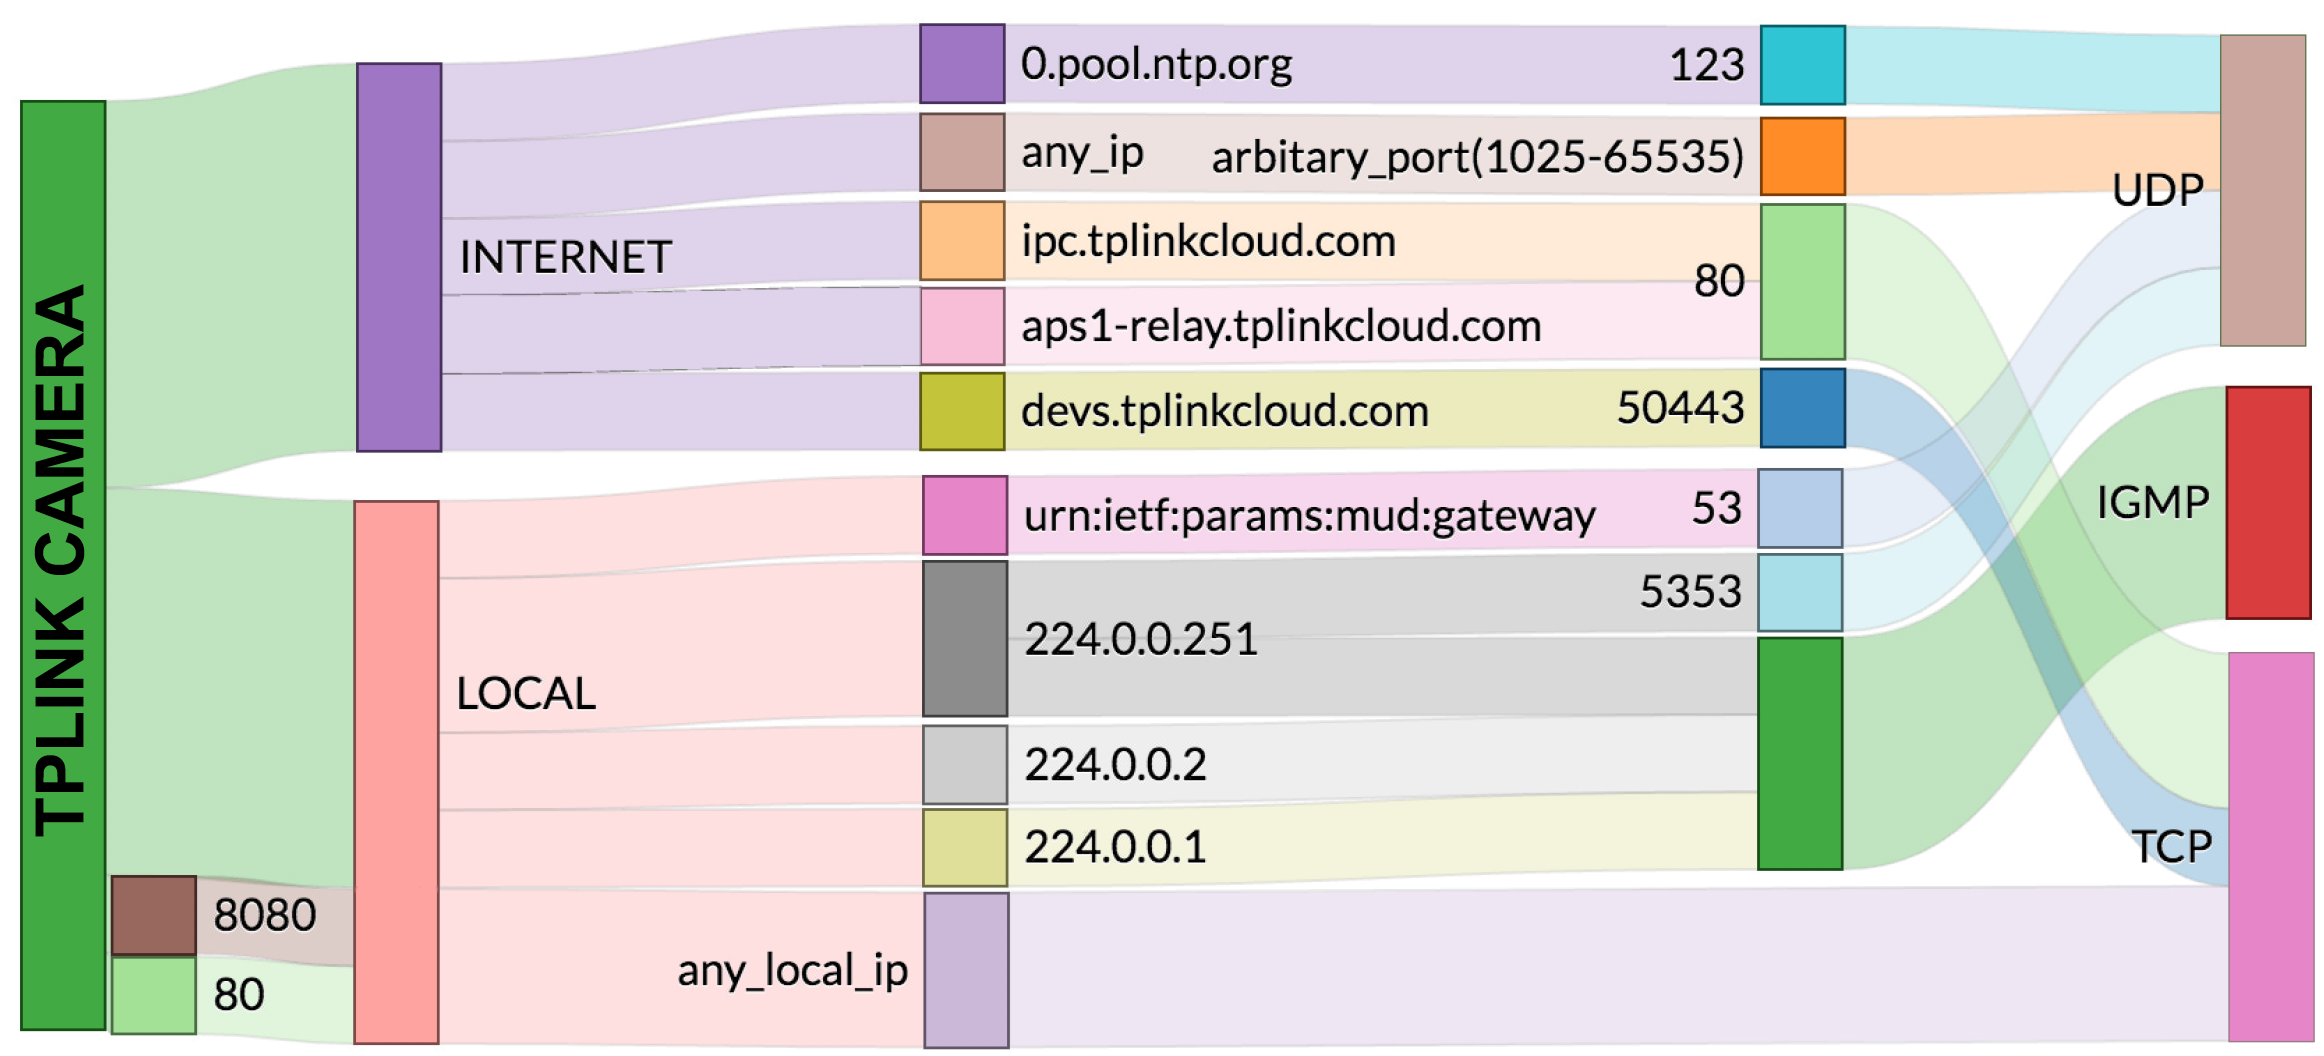
\includegraphics[width=0.7\linewidth]{Images/theory/tp_link_camera_mud}
	\caption{TP Link Camera MUD profile \cite{UNSWMUD2024}.}
	\label{fig:tplinkcameramud}
\end{figure}

For example, it specifies that the device communicates with \textit{0.pool.ntp.org} over UDP port 123 to use the Netwrok Time Protocol (NTP) in order to keep the camera's internal clock synchronized. Or its use of TCP port 80 via \textit{ipc.tplinkcloud.com} and \textit{aps1-relay.tplinkcloud.com} possibly for basic API check-ins, relay negotiations or unencrypted telemetry with the manufacturer's cloud. 

For a forensic investigator, the principles behind MUD are foundational for behavioral reconstruction:

\begin{itemize}
	\item \textbf{Establishing the Normal Baseline:} MUD profiles define the exact network features (destination IP addresses, transport protocols, and port numbers) that constitute normal behaviour.
	
	\item \textbf{Anomaly Detection as an Event Trigger:} If an investigator analyzing a PCAP file observes traffic that violates these NIST-recommended baseline, it can be used as a high-fidelity timestamp for a forensic event.
	
	\item \textbf{State Transitions:} By understanding the approved architectural flow of a smart home environment as outlined by NIST, investigators can map sudden bursts in compliant traffic to specific physical state transitions or possible attacks. 
\end{itemize}

\subsubsection{Networks of 'Things' Data Flow (NIST SP 800-183)}
To accurately reconstruct a forensic timeline, an investigator must understand the underlying science of how IoT data moves. NIST Special Publication 800-183 \cite{NISTSP800183} establishes the foundational primitives of IoT architectures, modeling the ecosystem using five core components: Sensors, Aggregators, Communication Channels, eUtilities, and Decision Triggers. 

For forensic timeline reconstruction, this framework is vital because it formalizes the chronological flow of IoT events. It dictates that a physical event begins at the Sensor, is encapsulated into packets traveling via a specific Communication Channel (the network), is routed by an Aggregator (the gateway), and ultimately results in a Decision Trigger (a physical actuation). Investigators can use this theoretical data flow model to map chronological packet sequences in a PCAP file directly back to the physical sequence of events occurring in the smart home.

Finally, while NIST guidelines are designed for security enforcement, risk management following a manufacturer oriented point of view, they provide the theoretical base required for forensic analysis. They confirm that IoT network traffic is intended to be highly structured and restricted, ensuring that the network feature extraction methods proposed in this research can reliably isolate specific device behaviours from benign background noise.


\subsection{IoT Forensic Frameworks}
As it has been previously been highlighted in previous sections, the academic and cybersecurity communities have recognized the inadequacy of classical forensic models. Consequently, numerous researchers have proposed specialized IoT forensic frameworks designed to navigate the highly distributed nature of these ecosystems. This subsections aims to review the state-of-the art frameworks to understand the current capabilities of digital investigators and to identify the gaps that this research seeks to address.

Current IoT forensic existing frameworks can generally be categorized into three approaches: Device-Centric, Cloud-Centric and Network-Centric model.

\subsubsection{Device and Cloud-Centric Frameworks}

First steps to formalize IoT investigations specially relied on extending traditional computing methodologies to smart devices.  Forensic-Aware IoT (FAIoT) model \cite{7207364}, is a clear example of this case. This framework advocates for a secure by design approach, arguing that forensic readiness must be directly built into the IoT infrastructure. In this schema, edge devices do not merely execute commands, they continuosly generate cryptographically signed operantional logs. Then, using Public Key Infrastructure (PKI) and secure hashing algorithms, devices immediately push these authenticated logs to a centralized and immutable repository known as the Secure Evidence Cloud (SEC). 

From the theoretical point of view, FAIoT directly neutralizes the hardware limitation of IoT devices by continuously offloading logs to the SEC. This ensures that data is preserved even if the physical edge device is rebooted, destroyed or compromised by an attacker. In addition, the SEC acts as a tamper-proof vault accessible to law enforcement via read-only APIs (non-repudiation and integrity). This ensures that the extracted timeline of events for an investigation has been not altered, satisfying the legal requirements for digital evidence admissibility. 

Another example is the multi-tiered framework proposed by Kebande and Ray \cite{Kebande2016}. This schema divides the investigation into specific zones (the Edge/Device Zone, the Network Zone, and the Cloud Zone), suggesting that investigators should acquire evidence from the physical device's flash memory or subpoena the vendor's cloud servers. This framework adapts established incident response standards such as ISO 27043 into a layered methodology, where the investigation landscape is divided into three distinct operational zones. 

\begin{itemize}
	\item \textbf{Edge Zone:} Groups the devices where investigation relies on classical hardware forensics attempting to extract residual state data from volatile memory (RAM), dump priopetary firmware via physical ports or analyze the limited local flash storage.
	\item \textbf{Network Zone:} Represents the communications channels and localized routing hardware (Smart Home Gateway). Evidence gathering focuses on intercepting in-transit data, capturing network packet traces (PCAPs) and analyzing protocol flows to reconstruct device-to-device or device-to-cloud communications.
	\item \textbf{Cloud Zone:} Ultimate centralized repository for device telemetry. This zone gathers vendor controlled data centers and APIs. The forensic efforts related to this zone involve acquiring long term historical data, user account activities, aggregated event logs...
\end{itemize}

This multilayered framework does noy treat the IoT incident as a single isolated event, since it forces the analyst to map the entire evidence trail from the physical trigger at the Edge, passing through the routing mechanisms at the network zone until the final persistent storage in the Cloud.

While theoretically sound, these frameworks suffer from practical limitations in real world scenarions:

\begin{itemize}
	\item \textbf{Manufacturer Reliance:} Frameworks like FAIoT require manufacturers to proactively build forensic logging into the devices, a practice that is economically and computationally prohibitive for IoT devices in general. 
	\item \textbf{Jurisdictional and Cloud Barriers:} Relying on the Cloud Zone requires legal consent from international cloud providers like AWS or TP-Link servers among others. This is a process that is exceedingly slow and often impossible for localized incident response.
	\item \textbf{Data Volatility:} As established in previous sections, by the time an investigator physically reaches the Edge Zone to attempt memory extraction, the volatile RAM containing the cryptographic keys and recent event states has typically been overwritten or lost to a reboot.
\end{itemize}

\subsubsection{Network-Centric Frameworks and the Remaining Gap}
Recognizing the physical and legal barriers of the Device and Cloud zones, modern forensic research has increasingly pivoted to the Network zone. Network-centric frameworks operate on the premise that local gateway is the only reliable and accessible point for evidence acquisition, since it is the chokepoint for all IoT communications. Because edge devices must route their traffic through this centralized hub to reach the wider internet or interact with peer devices, the gateway becomes the most reliable and accessible point for continuous evidence acquisition.

However, while the current body of literature broadly acknowledges the necessity of network packet capture (PCAP) in IoT investigations, a significant methodological shortcoming persists. Existing frameworks overwhelmingly focus on \textit{Device Identification}. This is the static process of fingerprinting a device's specific make, model, and operating system. While cataloging the hardware is a necessary preliminary step, these frameworks generally fail to address \textit{Behavioral Reconstruction}. They lack the capability to dynamically infer what the device is physically doing at a specific millisecond, such as distinguishing between a smart camera sitting idle, actively streaming video, or undergoing a malicious remote reboot. Furthermore, many legacy network forensic models still fundamentally rely on the assumption of plaintext communications, heavily utilizing Deep Packet Inspection (DPI) to simply read cleartext HTTP or MQTT payloads to determine device actions.

This reliance on DPI renders these legacy frameworks effectively obsolete in contemporary smart environments. Because modern IoT implementations overwhelmingly enforce robust encryption standards, such as TLS and DTLS (NISTIR 8259A), the payload contents are mathematically inaccessible to the investigator. Consequently, this raises the following problematic situation: investigators can successfully capture the encrypted network traffic, but they lack a standardized, step-by-step methodology to translate the remaining flow metadata—such as packet lengths, inter-arrival times, and throughput volumes—back into a reliable, chronological timeline of physical device events. Bridging this specific gap, without relying on payload decryption or physical device access, forms the primary objective of this research.

\subsubsection{Conclusion and Justification of Proposed Methodology}
The theoretical state of the art review presented in this subsection demonstrates a clear deficit in modern digital forensics. The inherent volatility of IoT hardware renders physical extraction unreliable, while the adoption of encryption neutralizes traditional network payload analysis. Although theoretical guidelines vestablish how devices \textit{should} behave, investigators lack a practical, passive methodology to definitively prove how they \textit{did} behave during a cyberattack.

To bridge this semantic gap, the subsequent chapters of this project will introduce, develop, and validate a novel methodology for IoT behavioral reconstruction. By strictly utilizing passive feature extraction on encrypted network traffic within a simulated smart home environment, this research aims to provide investigators with a reliable toolset for generating chronological forensic timelines without requiring device-level access or payload decryption.

